\documentclass[aspectratio=169]{beamer}

% Tema minimalista
\usetheme{metropolis} 

% Configuração de Cores: Fundo Branco e Detalhes Pretos
\setbeamercolor{background canvas}{bg=white}
\setbeamercolor{normal text}{fg=black}
\setbeamercolor{frametitle}{bg=white, fg=black}
\setbeamercolor{title}{fg=black}
\setbeamercolor{subtitle}{fg=gray}
\setbeamercolor{progress bar}{fg=black, bg=gray!30}
\setbeamercolor{alerted text}{fg=black}
\setbeamercolor{example text}{fg=black}

% Pacotes para português
\usepackage[utf8]{inputenc}
\usepackage[T1]{fontenc}
\usepackage[brazil]{babel}
\usepackage{tikz}
\usetikzlibrary{arrows.meta, positioning}
\usepackage[american]{circuitikz}
\usepackage{pgfplots}
\pgfplotsset{compat=1.18}
\usepackage{newtxtext,newtxmath}



% Configurações globais para as etiquetas de tensão e corrente
\ctikzset{
    voltage/distance from node=1, % Distância dos sinais +/- dos nós
    current/distance from node=0.5, % Distância das setas de corrente
    voltage/american plus=+,
    voltage/american minus=-,
    }


% Informações da Apresentação
\title{Identificação e controle aplicado a Conversores de Potência CC-CC}
\subtitle{topologia BUCK}


\author{
  \textbf{Discente:} Luiz Felipe Souza de Lima Silva \\[1em]
  \textbf{Orientador:} Prof. Raphael Texeira
}
\institute{Universidade Federal do Pará - CAMTUC }
\date{\today}



\begin{document}
{
  \logo{%
    \begin{tikzpicture}[remember picture, overlay]
      \node[anchor=north east, inner sep=10pt] at (current page.north east) {%
        
\includegraphics[height=1.2cm]{loguf.png}%
      };
    \end{tikzpicture}%
  }
  \begin{frame}
      \titlepage
  \end{frame}
}

% Slide de Título
\begin{frame}
  \titlepage
\end{frame}

% Slide de Sumário
\begin{frame}{Sumário}
  \tableofcontents
\end{frame}


% Slide com Lista
\begin{frame}{Objetivos específicos}
  \begin{itemize}
    \item Descrever o princípio de operação dos conversores CC-CC;
    \item Listar os tipos de conversor CC-CC;
    \item Modelar o circuito BUCK de acordo com as especificações de funcionamento;
    \item Obter a função de transferência da planta de acordo com o modelo;
    \item Obter um modelo via Identificação/modelagem em caixa preta;
    \item Projeto e discretização de controladores PID digitais;
    \item \textbf{Desenvolvimento de estratégias de Controle Preditivo Baseado em Modelo (MPC);}
  \end{itemize}
\end{frame}

\section{Introdução a Conversores CC-CC}


%PrimeiroSLIDE=============================================================================================================================================

\begin{frame}{Introdução}
\setbeamercolor{block title}{bg=black, fg=white}
  \setbeamercolor{block body}{bg=gray!10, fg=black}
  
\begin{block}{Conceito:}
    Um conversor CC pode ser considerado o equivalente CC de um transformador CA, e assim como o transformador, ele pode ser usado para baixar ou elevar uma fonte de tensão CC.
  \end{block}
    
\end{frame}

\begin{frame}{Relação entrada e saída}
  \begin{figure}[htbp]
    \centering
    \begin{tikzpicture}[x=1cm, y=1cm, >=Stealth]
      
      % Bloco central
      \draw[thick] (0,0) rectangle (3,2);
      \draw[thick] (0,0) -- (3,2);
      
      % Textos dentro do bloco (CC / CC)
      \node at (0.8, 1.3) {CC};
      \node at (2.2, 0.7) {CC};
      
      % Terminais de Entrada (Esquerda)
      % Linha superior de entrada
      \draw (-1.5, 1.5) -- (0, 1.5);
      \draw[fill=white] (-1.5, 1.5) circle (1.5pt);
      
      % Corrente i_s com seta
      \draw[->] (-0.8, 1.5) -- (-0.3, 1.5);
      \node[above] at (-0.55, 1.5) {$i_s$};
      
      % Tensão v_s e polaridades (+ / -)
      \node at (-1.1, 1.3) {$+$};
      \node at (-1.1, 0.3) {$-$};
      \node at (-1.5, 0.8) {$v_s$};
      
      % Linha inferior de entrada
      \draw (-1.5, 0.5) -- (0, 0.5);
      \draw[fill=white] (-1.5, 0.5) circle (1.5pt);

      % Terminais de Saída (Direita)
      % Linha superior de saída
      \draw (3, 1.5) -- (4.5, 1.5);
      \draw[fill=white] (4.5, 1.5) circle (1.5pt);
      
      % Tensão v_o e polaridades (+ / -)
      \node at (4.1, 1.3) {$+$};
      \node at (4.1, 0.3) {$-$};
      \node at (4.5, 0.8) {$v_o$};
      
      % Linha inferior de saída
      \draw (3, 0.5) -- (4.5, 0.5);
      \draw[fill=white] (4.5, 0.5) circle (1.5pt);

      % Legenda inferior
      \node at (1.5, -0.4) {Relação Entrada Saída};

    \end{tikzpicture}
  \end{figure}
\end{frame}


\begin{frame}{Reguladores chaveados e classificação}

Os conversores CC podem ser utilizados como reguladores chaveados (switching-mode regulators) a fim de converter uma tensão CC. \\

 Topologias básicas de regulador chaveado:
 
\begin{enumerate}
    \item Reguladores buck
    \item Reguladores boost 
    \item Reguladores buck-boost
\end{enumerate}
    
\end{frame}


%SEGUNDOSLIDE=============================================================================================================================================

\section{Conversores CC-CC tipo buck}

\begin{frame}{Principio de operação}
    O principio de operação fundamental do buck é como um abaixador.\\

    
    - Seja o seguinte esquema elétrico: \\
    
\begin{columns}[c] % Alinhamento vertical centralizado
        
        % --- COLUNA 1: CIRCUITO ---
        \begin{column}{0.48\textwidth}
            \centering
            \begin{tikzpicture}[scale=0.75, transform shape]
                
                % Terminais e Coordenadas
                \coordinate (t_in_top) at (0, 3);
                \coordinate (t_in_bot) at (0, 0);
                \coordinate (sw_in) at (2, 3);
                \coordinate (sw_out) at (3.5, 3);
                \coordinate (t_out_top) at (5, 3);
                \coordinate (t_out_bot) at (5, 0);
                
                % Linha inferior (retorno)
                \draw[thick] (t_in_bot) to[short] (t_out_bot);
                
                % Linha superior (entrada e seta de corrente)
                \draw[thick] (t_in_top) to[short, i^>={}, name=isrc] (sw_in);
                    
                % Chave (SW)
                \node[circ] at (sw_in) {};
                \node[circ] at (sw_out) {};
                \draw[thick] (sw_in) -- ++(1.3, 0.45);
                \draw[->, >=latex, semithick] ($ (sw_in) + (1.1, 0.5) $) arc (40:0:1) ;
                
                \node[below=1.5em] at ($ (sw_in)!0.5!(sw_out) $) {\small $t = 0$};
                \node[below=2.8em] at ($ (sw_in)!0.5!(sw_out) $) {\normalsize $SW$};
                
                % Linha superior (saída e seta de corrente)
                \draw[thick] (sw_out) to[short, i^>=$i_o$, name=iload] (t_out_top);
                    
                % Resistor de carga (R)
                \draw[thick] (t_out_top) to[R, l=$R$] (t_out_bot);
                    
                % Etiquetas de Entrada (V_s)
                \node[left=3pt, below=5pt] at (t_in_top) {\normalsize $+$};
                \node[left=3pt, above=5pt] at (t_in_bot) {\normalsize $-$};
                \node[left=10pt] at ($ (t_in_top)!0.5!(t_in_bot) $) {\normalsize $V_s$};
                
                % Terminais abertos
                \draw (t_in_top) circle (2.5pt);
                \draw (t_in_bot) circle (2.5pt);
                \draw (t_out_top) circle (2.5pt);
                \draw (t_out_bot) circle (2.5pt);
                
                % Etiqueta do Conversor
                \node at (2.75, 4) {\normalsize};
                
            \end{tikzpicture}
        \end{column}

        % --- COLUNA 2: FORMA DE ONDA ---
        \begin{column}{0.52\textwidth}
            \centering
            \begin{tikzpicture}[scale=0.75, transform shape, >=latex]
                
                % Eixos v_o e t
                \draw[->] (0,0) -- (6,0) node[right] {$t$};
                \draw[->] (0,0) -- (0,2.5) node[right] {$v_o$};
                
                % Valores nos eixos
                \node[below left] at (0,0) {$0$};
                \node[left] at (0,1.5) {$V_s$};
                
                % Desenho da forma de onda (espessura maior)
                \draw[very thick] (0,1.5) -- (2.2,1.5) -- (2.2,0) -- (5,0) -- (5,1.5) -- (5.6,1.5);
                
                % Cotas de tempo interno (t1 e t2)
                \draw[<->] (0,0.75) -- (2.2,0.75) node[midway, fill=white, inner sep=2pt] {$t_1$};
                \draw[<->] (2.2,0.75) -- (5,0.75) node[midway, fill=white, inner sep=2pt] {$t_2$};
                
                % Linhas guias inferiores para o Período T
                \draw (0, -0.1) -- (0, -1);
                \draw[dashed] (2.2, 0) -- (2.2, -1);
                \draw (5, -0.1) -- (5, -1);
                
                % Cota do período (T)
                \draw[<->] (0,-0.8) -- (5,-0.8) node[midway, fill=white, inner sep=2pt] {$T$};

            \end{tikzpicture}
        \end{column}
        
    \end{columns}
    
\end{frame}

\begin{frame}{Cálculo da Tensão Média}
  \setbeamercolor{block title}{bg=black, fg=white}
  \setbeamercolor{block body}{bg=gray!10, fg=black}
  
  \begin{block}{Definição:}

    \[
V_0= \frac{1}{T} \int_{0}^{t_1} v_0 \, dt = \frac{t_1}{T} V_s = k V_s
\]

  \end{block}

  \begin{itemize}
    \item $V_0$ = Tensão saída;
    \item $T$ = Período;
    \item $k$ = Duty Cycle.
\end{itemize}

\end{frame}


\begin{frame}{Conversor buck}
    A partir do principio de operação apresentado é obtido que a tensão média de saída $V_0$ é menor do que a de entrada $Vs$ —   daí o nome “buck” (N. do tradutor: “patente menor em uma categoria militar”).
\end{frame}

\begin{frame}{Diagrama do Circuito buck}
  \begin{figure}[htbp]
    \centering
    \resizebox{\textwidth}{!}{%
    \begin{circuitikz}[>=latex, scale=1.0, transform shape]
        
        % Terminais de Entrada
        \draw (0, 3) node[ocirc] (in_plus) {};
        \draw (0, 0) node[ocirc] (in_minus) {};
        
        % Tensão Vs
        \node at (0, 1.5) {$V_s$};
        \node at (0, 2.7) {$+$};
        \node at (0, 0.3) {$-$};
        
        % Transistor Q1
        \node[npn, rotate=90] (q1) at (2.5, 3) {};
        \node[above, yshift=0.2cm] at (q1.center) {$Q_1$};
        
        % Fio de entrada e Seta de corrente i_s
        \draw (in_plus) -- (q1.collector);
        \draw[->] (0.8, 3) -- (1.3, 3);
        \node[above] at (1.05, 3) {\small $i_s, I_s$};
        
        % Linha de terra principal (inferior)
        \draw (in_minus) -- (12, 0);
        
        % Nó de comutação
        \draw (q1.emitter) -- (4, 3);
        \node[circle, fill, inner sep=1pt] at (4, 3) {};
        
        % Diodo Dm
        \draw (4, 0) to[D] (4, 3);
        \node[right] at (4.2, 1.5) {$D_m$};
        \node[circle, fill, inner sep=1pt] at (4, 0) {};
        
        % Indutor L
        \draw (4, 3) to[L] (7.5, 3);
        \node[above] at (5.75, 3.4) {$L$};
        \node at (5.75, 4.0) {$e_L$};
        \node at (5.0, 3.8) {$+$};
        \node at (6.5, 3.8) {$-$};
        
        % Corrente i_L (antes do indutor)
        \draw[->] (4.3, 3) -- (4.8, 3);
        \node[below] at (4.55, 3) {\small $i_L, I_L$};
        
        % Ponto de Realimentação e Seta i_L (depois do indutor)
        \node[circle, fill, inner sep=1pt] (fb_node) at (7.5, 3) {};
        \draw (7.5, 3) -- (8.5, 3);
        \draw[->] (7.7, 3) -- (8.2, 3);
        \node[above] at (7.95, 3) {\small $i_L$};
        
        % Capacitor C (sem rótulos de tensão, corrente ou nome)
        \draw (8.5, 3) to[C] (8.5, 0);
        \node[circle, fill, inner sep=1pt] at (8.5, 3) {};
        \node[circle, fill, inner sep=1pt] at (8.5, 0) {};
        
        % Bloco de Carga
        \draw (8.5, 3) -- (10.5, 3);
        \node[draw, rectangle, minimum width=1.4cm, minimum height=0.9cm, fill=white] (load) at (10.5, 1.5) {Carga};
        \draw (10.5, 3) -- (load.north);
        \draw (load.south) -- (10.5, 0);
        \node[circle, fill, inner sep=1pt] at (10.5, 3) {};
        \node[circle, fill, inner sep=1pt] at (10.5, 0) {};
        
        % Seta corrente i_o da carga
        \draw[->] (10.5, 2.6) -- (10.5, 2.1);
        \node[right] at (10.6, 2.35) {\small $i_o, I_a$};
        
        % Terminais de Saída
        \draw (10.5, 3) -- (12, 3) node[ocirc] {};
        \draw (10.5, 0) -- (12, 0) node[ocirc] {};
        
        % Tensão vo
        \node at (12.2, 1.5) {$v_o, V_a$};
        \node at (12, 2.7) {$+$};
        \node at (12, 0.3) {$-$};
        
        % Bloco de Controle
        \node (ctrl) at (2.5, 0.75) [draw, rectangle, minimum width=2.0cm, minimum height=1cm, fill=white] {Controle};
        
        % Conexão Controle -> Base Q1
        \draw[-latex] (ctrl.north) -- (q1.base);
        
        % Fio de Realimentação
        \draw (fb_node) -- (7.5, 0.75) -- (4.2, 0.75);
        \draw (4.2, 0.75) arc[start angle=0, end angle=180, radius=0.2cm];
        \draw[-latex] (3.8, 0.75) -- (ctrl.east);
        
        % Legenda Inferior
        \node at (6.0, -0.75) [font=\small] { Diagrama circuito elétrico buck };

    \end{circuitikz}%
    }
  \end{figure}
\end{frame}

\begin{frame}{Modos de operação}
  \begin{figure}[htbp]
    \centering
    \begin{columns}[T] % Alinhamento superior das colunas
      
      % --- COLUNA 1: Modo 1 ---
      \begin{column}{0.48\textwidth}
        \centering
        \resizebox{\linewidth}{!}{%
        \begin{circuitikz}[>=latex, scale=1.0, transform shape]
            % Terminais de Entrada
            \draw (0, 2.5) node[ocirc] (in_plus) {};
            \draw (0, 0) node[ocirc] (in_minus) {};
            \node at (0, 1.25) {$V_s$};
            \node at (0, 2.2) {$+$};
            \node at (0, 0.3) {$-$};
            
            % Indutor L com seta is = iL
            \draw (in_plus) -- (1.0, 2.5);
            \draw[->] (1.0, 2.5) -- (1.6, 2.5);
            \node[above] at (1.3, 2.5) {\small $i_s = i_L$};
            
            \draw (1.6, 2.5) to[L] (4.5, 2.5);
            \node[above] at (3.05, 2.9) {$L$};
            
            % Terra inferior
            \draw (in_minus) -- (7.0, 0);
            
            % Nó de saída/capacitor
            \node[circle, fill, inner sep=1pt] (node_c) at (4.5, 2.5) {};
            \draw (4.5, 2.5) -- (6.0, 2.5);
            
            % Capacitor C
            \draw (4.5, 2.5) to[C] (4.5, 0);
            \node[right] at (4.7, 1.25) {$v_c$};
            \node at (4.2, 2.1) {$+$};
            \node at (4.2, 0.4) {$-$};
            \draw[->] (4.5, 2.1) -- (4.5, 1.6);
            \node[right] at (4.6, 1.85) {\small $i_c$};
            \node[circle, fill, inner sep=1pt] at (4.5, 0) {};
            
            % Carga
            \node[draw, rectangle, minimum width=1.2cm, minimum height=0.8cm, fill=white] (load) at (6.0, 1.25) {Carga};
            \draw (6.0, 2.5) -- (load.north);
            \draw (load.south) -- (6.0, 0);
            \draw[->] (6.0, 2.1) -- (6.0, 1.7);
            \node[right] at (6.1, 1.9) {\small $i_o = I_a$};
            
        \end{circuitikz}%
        }
        \vspace{0.1cm}
        \small Modo 1 - Chave on
      \end{column}
      
      % --- COLUNA 2: Modo 2 ---
      \begin{column}{0.48\textwidth}
        \centering
        \resizebox{\linewidth}{!}{%
        \begin{circuitikz}[>=latex, scale=1.0, transform shape]
            % Fio esquerdo com Diodo Dm
            \draw (0, 0) -- (0, 2.5);
            \draw (0, 0) node[circle, fill, inner sep=1pt] {};
            \draw (0, 2.5) node[circle, fill, inner sep=1pt] {};
            \draw (0, 0) to[D] (0, 2.5);
            \node[right] at (0.2, 1.25) {$D_m$};
            
            % Indutor L com seta iL
            \draw (0, 2.5) -- (1.6, 2.5);
            \draw[->] (0.5, 2.5) -- (1.1, 2.5);
            \node[above] at (0.8, 2.5) {\small $i_L$};
            
            \draw (1.6, 2.5) to[L] (4.5, 2.5);
            \node[above] at (3.05, 2.9) {$L$};
            
            % Terra inferior
            \draw (0, 0) -- (7.0, 0);
            
            % Nó de saída/capacitor
            \node[circle, fill, inner sep=1pt] (node_c2) at (4.5, 2.5) {};
            \draw (4.5, 2.5) -- (6.0, 2.5);
            
            % Capacitor C
            \draw (4.5, 2.5) to[C] (4.5, 0);
            \node[right] at (4.7, 1.25) {$v_c$};
            \node at (4.2, 2.1) {$+$};
            \node at (4.2, 0.4) {$-$};
            \draw[->] (4.5, 2.1) -- (4.5, 1.6);
            \node[right] at (4.6, 1.85) {\small $i_c$};
            \node[circle, fill, inner sep=1pt] at (4.5, 0) {};
            
            % Carga
            \node[draw, rectangle, minimum width=1.2cm, minimum height=0.8cm, fill=white] (load2) at (6.0, 1.25) {Carga};
            \draw (6.0, 2.5) -- (load2.north);
            \draw (load2.south) -- (6.0, 0);
            \draw[->] (6.0, 2.1) -- (6.0, 1.7);
            \node[right] at (6.1, 1.9) {\small $i_o = I_a$};
            
        \end{circuitikz}%
        }
        \vspace{0.1cm}
        \small Modo 2 - chave off
      \end{column}

    \end{columns}
    
    \vspace{0.3cm}
    \small  Circuitos 
  \end{figure}
\end{frame}

\begin{frame}{Modelo Matemático buck}
  \setbeamercolor{block title}{bg=black, fg=white}
  \setbeamercolor{block body}{bg=gray!10, fg=black}
  
  \begin{block}{Conceito chave:}
    O Modelo do sistema é obtido através de um modelo médio, que é construído analisando cada um dos dois modos de operação.
  \end{block}
\end{frame}

\begin{frame}{Modelo buck}
  \setbeamercolor{block title}{bg=black, fg=white}
  \setbeamercolor{block body}{bg=gray!10, fg=black}
  
  \begin{block}{Definição do Modelo médio:}
    $$\dot{x}(t) = M_1 \cdot x(t) + M_2 \cdot u(t)$$
  \end{block}
\begin{itemize}
        \item $M_1$ e $M_2$ representam médias ponderadas das matrizes em cada modo de operação(ex: chave off e chave on).
        \item $k$ representa a razão cíclica (\textit{duty cycle}).
        \item $(1 - k)$ representa o complemento da razão cíclica.
    \end{itemize}

\end{frame}


%TerceiroSLIDE=============================================================================================================================================
\section{Análise do regulador buck no espaço de estados/Modelo}

% Slide com Bloco Destacado (Borda preta)
\begin{frame}{Análise no espaço de estados}
  \setbeamercolor{block title}{bg=black, fg=white}
  \setbeamercolor{block body}{bg=gray!10, fg=black}

 \begin{block}{Equação de Estado:}
   $$\dot{x}(t) = A \cdot x(t) + B \cdot u_1(t)$$
  \end{block}
\\
  - A partir da equação apresentada define-se a equação de estados para cada modo de operação
  \\

  \end{frame}

\begin{frame}{Análise no espaço de estados}

- A partir do modo de operação 1 - chave fechada:
\\


\begin{figure}[htbp]
    \centering
    \resizebox{0.5\textwidth}{!}{%
    \begin{circuitikz}[>=latex, scale=1.0, transform shape]
        
        % Fonte de Tensão u1 (à esquerda)
        \draw (0,0) to[V, v=$u_1$, invert] (0,3);
        \node at (-0.3, 2.3) {$+$};
        \node at (-0.3, 0.7) {$-$};
        
        
        % Seta de corrente x1 no topo esquerdo
        \draw[->] (1.0, 3) -- (1.6, 3);
        \node[above] at (1.3, 3) {\small $x_1$};
        
        % Indutor L no topo
        \draw (0, 3) -- (1.0, 3);
        \draw (1.6, 3) to[L] (4.5, 3);
        \node[above] at (3.05, 3.4) {$L$};
        
        % Terra/linha inferior
        \draw (0, 0) -- (6.0, 0);
        
        % Nó superior e Capacitor C
        \node[circle, fill, inner sep=1.2pt] at (4.5, 3) {};
        \draw (4.5, 3) to[C] (4.5, 0);
        \node[left] at (4.3, 1.5) {$$};
        \node[right] at (4.7, 1.5) {$x_2$};
        \node at (4.2, 2.1) {$+$};
        \node at (4.2, 0.4) {$-$};
        \node[circle, fill, inner sep=1.2pt] at (4.5, 0) {};
        
        % Linha superior direita e Resistor R
        \draw (4.5, 3) -- (6.0, 3);
        \draw (6.0, 3) to[R, l=$R$] (6.0, 0);
        
        % Legenda inferior
        \node at (3.0, -0.8) [font=\small] {(a) Circuito equivalente para o modo 1};

    \end{circuitikz}%
    }
  \end{figure}


\end{frame}
\begin{frame}{Análise no espaço de estados}
     \setbeamercolor{block title}{bg=black, fg=white}
  \setbeamercolor{block body}{bg=gray!10, fg=black}

\begin{block}{Equação de Estado modo 1}
\begin{center}
    
      $$\begin{bmatrix} 
        \dot{x}_1 \\ 
        \dot{x}_2 
      \end{bmatrix} = 
      \begin{bmatrix} 
        0 & -\frac{1}{L} \\ 
        \frac{1}{C} & -\frac{1}{RC} 
      \end{bmatrix}
      \begin{bmatrix} 
        x_1 \\ 
        x_2 
      \end{bmatrix} + 
      \begin{bmatrix} 
        \frac{1}{L} \\ 
        0 
      \end{bmatrix} u_1(t)$$
    \end{center}
  \end{block}
\end{frame}

\begin{frame}{Análise no espaço de estados}

- A partir do modo de operação 2 - chave aberta:

\\

\begin{figure}[htbp]
    \centering
    \resizebox{0.5\textwidth}{!}{%
    \begin{circuitikz}[>=latex, scale=0.75, transform shape]
        
        % Diodo S2 à esquerda (em pé, apontando para cima)
        \draw (0, 0) to[D, l_=$S_2$] (0, 3);
        \node[circle, fill, inner sep=1.2pt] at (0, 0) {};
        \node[circle, fill, inner sep=1.2pt] at (0, 3) {};
        
        % Seta de corrente x1 no topo esquerdo
        \draw[->] (1.0, 3) -- (1.6, 3);
        \node[above] at (1.3, 3) {\small $x_1$};
        
        % Indutor L no topo
        \draw (0, 3) -- (1.0, 3);
        \draw (1.6, 3) to[L] (4.5, 3);
        \node[above] at (3.05, 3.4) {$L$};
        
        % Terra/linha inferior
        \draw (0, 0) -- (6.0, 0);
        \node[circle, fill, inner sep=1.2pt] at (4.5, 0) {};
        
        % Nó superior e Capacitor C (sem a letra C, mantendo x2 e polaridades)
        \node[circle, fill, inner sep=1.2pt] at (4.5, 3) {};
        \draw (4.5, 3) to[C] (4.5, 0);
        \node[right] at (4.7, 1.5) {$x_2$};
        \node at (4.2, 2.1) {$+$};
        \node at (4.2, 0.4) {$-$};
        
        % Linha superior direita e Resistor R
        \draw (4.5, 3) -- (6.0, 3);
        \draw (6.0, 3) to[R, l=$R$] (6.0, 0);
        
        % Legenda inferior
        \node at (3.0, -0.8) [font=\small] {(b) Circuito equivalente para o modo 2};

    \end{circuitikz}%
    }
  \end{figure}


\end{frame}
\begin{frame}{Análise no espaço de estados}

\setbeamercolor{block title}{bg=black, fg=white}
  \setbeamercolor{block body}{bg=gray!10, fg=black}

  \begin{block}{Equação de Estado modo 2}
    \begin{center}
      $$\begin{bmatrix} 
        \dot{x}_1 \\ 
        \dot{x}_2 
      \end{bmatrix} = 
      \begin{bmatrix} 
        0 & -\frac{1}{L} \\ 
        \frac{1}{C} & -\frac{1}{RC} 
      \end{bmatrix}
      \begin{bmatrix} 
        x_1 \\ 
        x_2 
      \end{bmatrix} + 
      \begin{bmatrix} 
        0 \\ 
        0  
      \end{bmatrix} u_1(t)$$ 
    \end{center}
  \end{block}
    
\end{frame}

\begin{frame}{Análise no espaço de estados}

- Define-se então a Matriz ponderada para cada modo de operação:

    \setbeamercolor{block title}{bg=black, fg=white}
  \setbeamercolor{block body}{bg=gray!10, fg=black}

 \begin{block}{Equação de Estado modo 1}
\begin{center}
    
      $$\begin{bmatrix} 
        \dot{x}_1 \\ 
        \dot{x}_2 
      \end{bmatrix} = 
      \begin{bmatrix} 
        0 & -\frac{1}{L} \\ 
        \frac{1}{C} & -\frac{1}{RC} 
      \end{bmatrix}
      \begin{bmatrix} 
        x_1 \\ 
        x_2 
      \end{bmatrix} + 
      \begin{bmatrix} 
        \frac{1}{L} \\ 
        0 
      \end{bmatrix} u_1(t)$$
    \end{center}
    
\begin{center}
      $$M_1 = k \cdot A_1 + (1 - k) \cdot A_2$$
    \end{center}
    
  \end{block}

 
\end{frame}



\begin{frame}{Análise no espaço de estados}
    \setbeamercolor{block title}{bg=black, fg=white}
  \setbeamercolor{block body}{bg=gray!10, fg=black}

  \begin{block}{Equação de Estado modo 2}
    \begin{center}
      $$\begin{bmatrix} 
        \dot{x}_1 \\ 
        \dot{x}_2 
      \end{bmatrix} = 
      \begin{bmatrix} 
        0 & -\frac{1}{L} \\ 
        \frac{1}{C} & -\frac{1}{RC} 
      \end{bmatrix}
      \begin{bmatrix} 
        x_1 \\ 
        x_2 
      \end{bmatrix} + 
      \begin{bmatrix} 
        0 \\ 
        0  
      \end{bmatrix} u_1(t)$$ 
    \end{center}

    \begin{center}
      $$M_2 = k \cdot B_1 + (1 - k) \cdot B_2$$
    \end{center}
  \end{block}
  
\end{frame}



\begin{frame}{Análise no espaço de estados}
 \setbeamercolor{block title}{bg=black, fg=white}
  \setbeamercolor{block body}{bg=gray!10, fg=black}
  
- Portanto o Modelo médio:
\begin{block}{Modelo médio}
    \begin{center}
    $$\dot{x}(t) = M_1 \cdot x(t) + M_2 \cdot u_1(t)$$
    \end{center}

    \begin{center}
     
      \begin{bmatrix} 
        \dot{x}_1 \\ 
        \dot{x}_2 
      \end{bmatrix} = 
      \begin{bmatrix} 
        0 & -\frac{1}{L} \\ 
        \frac{1}{C} & -\frac{1}{RC} 
      \end{bmatrix}
      \begin{bmatrix} 
        x1 \\ 
        x_2 
      \end{bmatrix} + 
      \begin{bmatrix} 
        \frac{k}{L} \\ 
        0 
      \end{bmatrix} $u_1(t)$
    \end{center}
\end{block}

\end{frame}

\begin{frame}{Modelo Linearizado por Pequenos Sinais}
- Modelo Linearizado por pequenos sinais:

 \setbeamercolor{block title}{bg=black, fg=white}
  \setbeamercolor{block body}{bg=gray!10, fg=black}
  
    \begin{block}{Equações de Estado do Sistema Linearizado}
        \begin{equation*}
            \begin{cases}
                \dot{  \hat{x}}_1 = \dfrac{-u_1 \hat{k}(t)}{L} - \dfrac{\hat{x}_2(t)}{L} \\[1.2em]
                \dot{\hat{x}}_2 = \dfrac{\hat{x}_1(t)}{C} - \dfrac{\hat{x}_2(t)}{R \cdot C}
            \end{cases}
        \end{equation*}
    \end{block}

\end{frame}

\begin{frame}{Função de Transferência do Conversor}

 \setbeamercolor{block title}{bg=black, fg=white}
  \setbeamercolor{block body}{bg=gray!10, fg=black}
  
    \begin{block}{Relação Entrada-Saída no Domínio de Laplace}
        \begin{equation*}
            G(s) = \frac{y(s)}{u(s)} = \frac{x_2(s)}{k(s)}
        \end{equation*}

        \begin{figure}
        \centering
        \begin{tikzpicture}[
            auto,
            node distance=2.5cm,
            >=Stealth,
            block/.style={
                draw,
                rectangle,
                rounded corners,
                minimum height=1.5cm,
                minimum width=2.5cm,
                align=center,
                line width=0.8pt
            }
        ]
            % No central do sistema
            \node [block] (system) {$G(s)$};

            % Entrada (Seta da esquerda)
            \draw [->, line width=0.6pt] (system.west) ++(-3cm, 0) -- (system.west)
                node [midway, above] {$K(s)$ -- duty cycle};

            % Saida (Seta da direita)
            \draw [->, line width=0.6pt] (system.east) -- ++(3.5cm, 0)
                node [midway, above] {$x_2(s)$ Tensão em C};
        \end{tikzpicture}
    \end{figure}
    \end{block}

\end{frame}

\begin{frame}{Função de Transferência do Conversor Buck}

\setbeamercolor{block title}{bg=black, fg=white}
  \setbeamercolor{block body}{bg=gray!10, fg=black}
  
    \begin{block}{Modelo Analítico de Segunda Ordem/planta}
        \begin{equation*}
            G(s) = \frac{u_1}{s^2 \cdot CL + \dfrac{L \cdot s}{R} + 1}
        \end{equation*}
    \end{block}

\end{frame}

\section{Identificação do sistema}

\begin{frame}{Identificação}
    A partir da coleta de dados foi obtido um modelo do sistema, partindo da ideia de modelagem por identificação, tambem conhecida por modelagem em caixa preta. 
    
    \\
    \vspace{1cm}

    \begin{figure}
        \centering
        \begin{tikzpicture}[
            auto,
            node distance=2.5cm,
            >=Latex,
            % Estilo do bloco central
            block/.style={
                draw=black,
                fill=white,
                rectangle,
                minimum width=3cm,
                minimum height=2cm,
                line width=1pt,
                align=center
            },
            % Estilo das linhas/setas de sinal
            signal/.style={
                draw=black,
                ->,
                line width=1pt
            }
        ]

            % Bloco central com interrogação
            \node [block] (system) {\sffamily\Huge ?};

            % Pontos invisíveis para delimitar as setas
            \node [left=of system] (input) {};
            \node [right=of system] (output) {};

            % Setas e rótulos
            \draw [signal] (input) -- node[above, font=\sffamily\large\bfseries] {ENTRADA} (system);
            \draw [signal] (system) -- node[above, font=\sffamily\large\bfseries] {SAÍDA} (output);

        \end{tikzpicture}
        %\caption{Representação genérica de um sistema.}
    \end{figure}

\end{frame}

\begin{frame}[fragile]{Identificação}

A Escolha do modelo:

\setbeamercolor{block title}{bg=black, fg=white}
  \setbeamercolor{block body}{bg=gray!10, fg=black}
  
    \begin{block}{Modelo ARX}
        \begin{itemize}
            \item Equações de diferenças ARX, pode ser definida por:
        \end{itemize}
        
        \begin{equation*}
            y(k) = \sum_{i=1}^{n} a_i y(k - i) + \sum_{j=1}^{n} b_j y(k - i)
        \end{equation*}
    \end{block}
- Para dois coeficientes de entrada e saída, teremos:

\end{frame}

\begin{frame}{Identificação}
\setbeamercolor{block title}{bg=black, fg=white}
  \setbeamercolor{block body}{bg=gray!10, fg=black}
  
    \begin{block}{Representação Matricial do Modelo ARX}
        \begin{equation*}
            A \cdot X = Y
        \end{equation*}

        \begin{equation*}
            \underbrace{%
                \begin{bmatrix}
                    y(3) \\
                    y(4) \\
                    \vdots \\
                    y(N)
                \end{bmatrix}%
            }_{Y}
            =
            \underbrace{%
                \begin{bmatrix}
                    y(2) & y(1) & u(2) & u(1) \\
                    y(3) & y(2) & u(3) & u(2) \\
                    \vdots & \vdots & \vdots & \vdots \\
                    y(N-1) & y(N-2) & u(N-1) & u(N-2)
                \end{bmatrix}%
            }_{A}
            \underbrace{%
                \begin{bmatrix}
                    a_1 \\
                    a_2 \\
                    b_1 \\
                    b_2
                \end{bmatrix}%
            }_{X}
        \end{equation*}
    \end{block}

    \begin{block}{Solução para o Vetor de Parâmetros}
        \begin{equation*}
            X = (A^T \cdot A)^{-1} \cdot A^T \cdot Y
        \end{equation*}
    \end{block}

\end{frame}

\begin{frame}[fragile]{Função de Transferência Discreta}
\setbeamercolor{block title}{bg=black, fg=white}
  \setbeamercolor{block body}{bg=gray!10, fg=black}
  
    \begin{block}{Modelo Discreto Identificado:}
        Portanto, obtem-se:
        
        \begin{equation*}
            G(q) = \frac{b1 q^{-1} + b2 q^{-2}}{1 - a1 q^{-1} - a2 q^{-2}}
        \end{equation*}

        \vspace{0.5em}
        O modelo discreto obtido pode ser comparado com um modelo ideal.
    \end{block}

\end{frame}

\begin{frame}{Resultados do Modelo Identificado}

    \begin{figure}
        \centering
        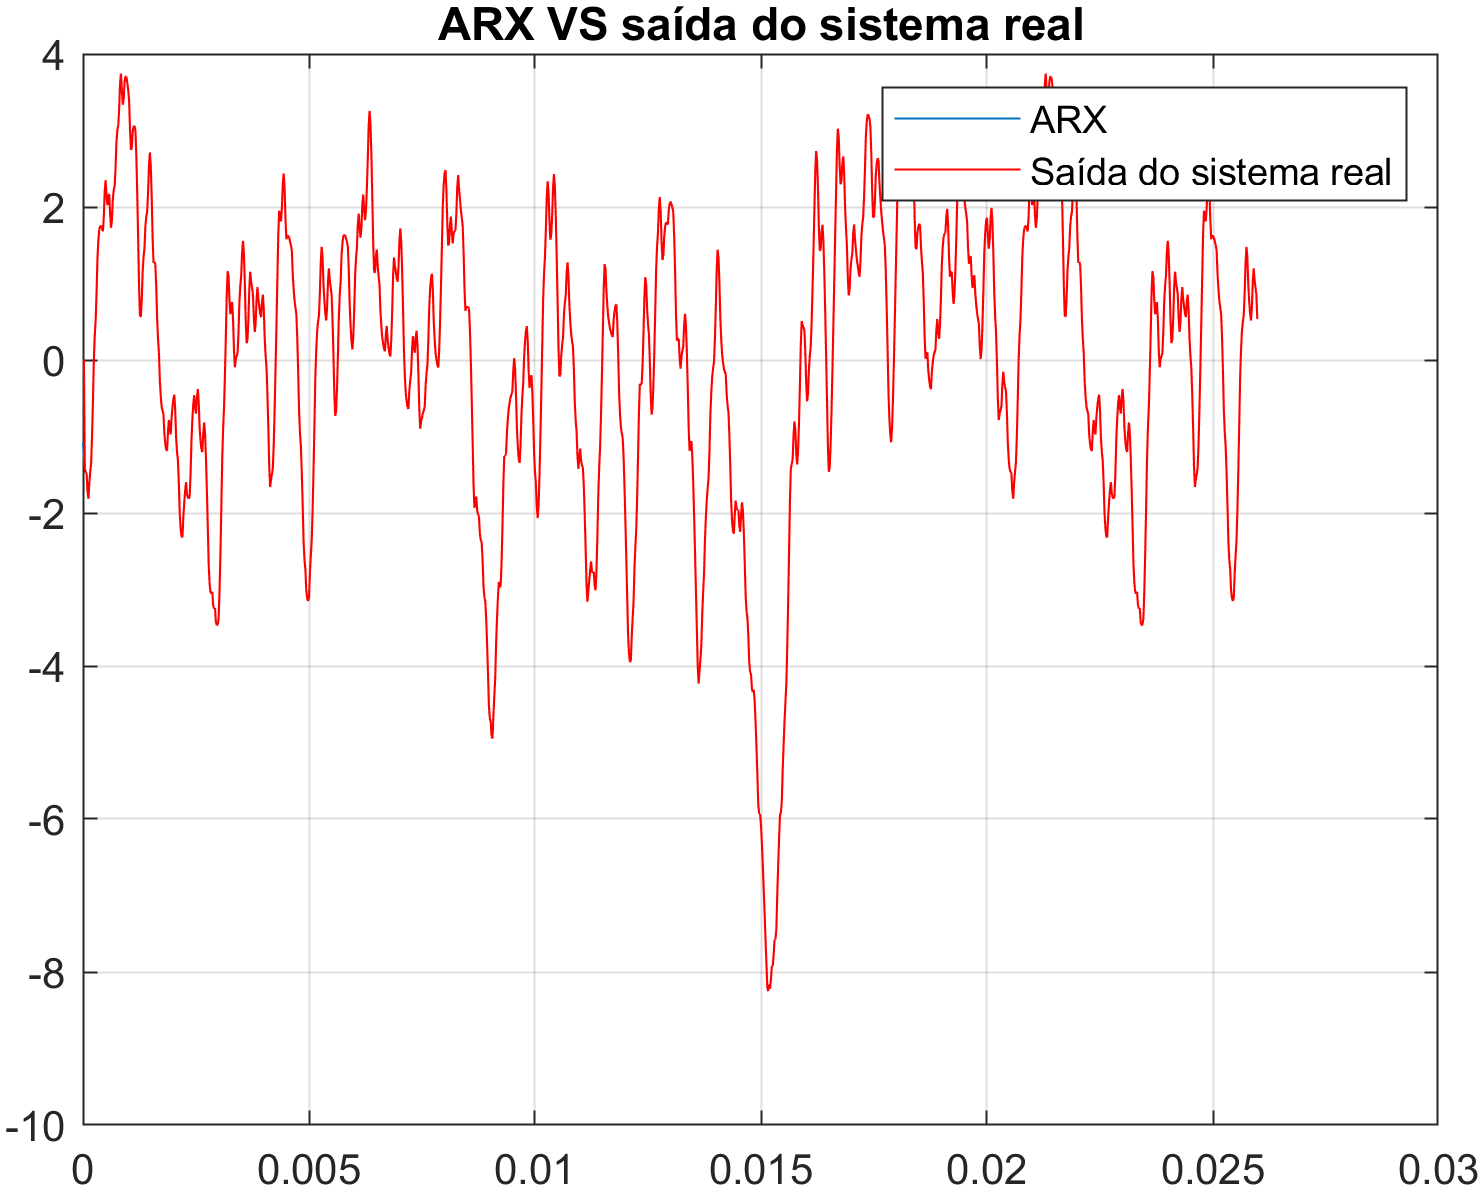
\includegraphics[width=0.65\textwidth]{comparacao_arx.png}
        %\caption{Comparação temporal entre o modelo ARX e a resposta real.}
    \end{figure}

\end{frame}

\section{Projeto e Sintonia de Controlador PID via Lugar Geométrico das Raízes (LGR)}

\begin{frame}{Introdução à Teoria de Controle}

- Conceito de Malha Fechada:

\begin{figure}[h]
\centering
\scalebox{0.8}{
\begin{tikzpicture}[
    >=Latex,
    block/.style={draw, rectangle, minimum height=1.2cm, minimum width=2.2cm, align=center, font=\small},
    node distance=3.2cm
]

    % Blocos e pontos de referência
    \node (input) {};
    \node[block, right of=input, node distance=2.5cm] (ctrl) {Controlador};
    \node[block, right of=ctrl, node distance=3.5cm] (plant) {Planta\\ou\\Processo};
    \node[right of=plant, node distance=3.0cm] (output) {};
    
    % Elemento de Medição na realimentação
    \node[block, below of=ctrl, node distance=2.2cm, xshift=1.75cm] (sensor) {Elemento\\de\\Medição};

    % Conexões da linha direta
    \draw[->, thick] (input) -- node[above, font=\small] {entrada} (ctrl);
    \draw[->, thick] (ctrl) -- (plant);
    \draw[->, thick] (plant) -- node[coordinate] (branch) {} node[above, font=\small, pos=0.7] {saída} (output);

    % Malha de realimentação
    \draw[->, thick] ($(plant)!0.5!(output)$) |- (sensor);
    \draw[->, thick] (sensor) -| (ctrl);

\end{tikzpicture}
}
\end{figure}

\end{frame}


 \begin{frame}{Controlador PID}

\setbeamercolor{block title}{bg=black, fg=white}
  \setbeamercolor{block body}{bg=gray!10, fg=black}
  
\begin{block}{Definicao}
    $$C(s) = K_p + \frac{K_i}{s} + K_d \cdot s$$
    
    \vspace{0.2cm}
    \textbf{Onde:}
    \begin{itemize}
        \item $K_p \rightarrow$ ganho proporcional
        \item $K_i \rightarrow$ ganho integral
        \item $K_d \rightarrow$ ganho derivativo
    \end{itemize}
\end{block}

- Escolha do controlador ideal para o problema.

- Desafio de Sintonia: Ajustar os três ganhos simultaneamente para balancear velocidade de resposta, estabilidade e sobresinal.

\end{frame}

\begin{frame}{Função de Transferência da Planta}

\setbeamercolor{block title}{bg=black, fg=white}
  \setbeamercolor{block body}{bg=gray!10, fg=black}
\begin{block}{Modelo Analítico da Planta $G(s)$:}
    $$G(s) = \frac{\frac{V_s}{L \cdot C}}{s^2 + \frac{1}{R \cdot C} \cdot s + \frac{1}{L \cdot C}}$$
\end{block}

\begin{block}{Função de Transferência Substituída com todos termos:}
    $$G(s) = \frac{1{,}532 \times 10^9}{s^2 + 24000 \cdot s + 51{,}06 \times 10^6}$$
\end{block}

\end{frame}

\begin{frame}{Escolha do Controlador}

         Utilizou-se a ferramenta \texttt{controlSystemDesigner} do MATLAB para a análise e sintonia.

\begin{figure}
        \centering
        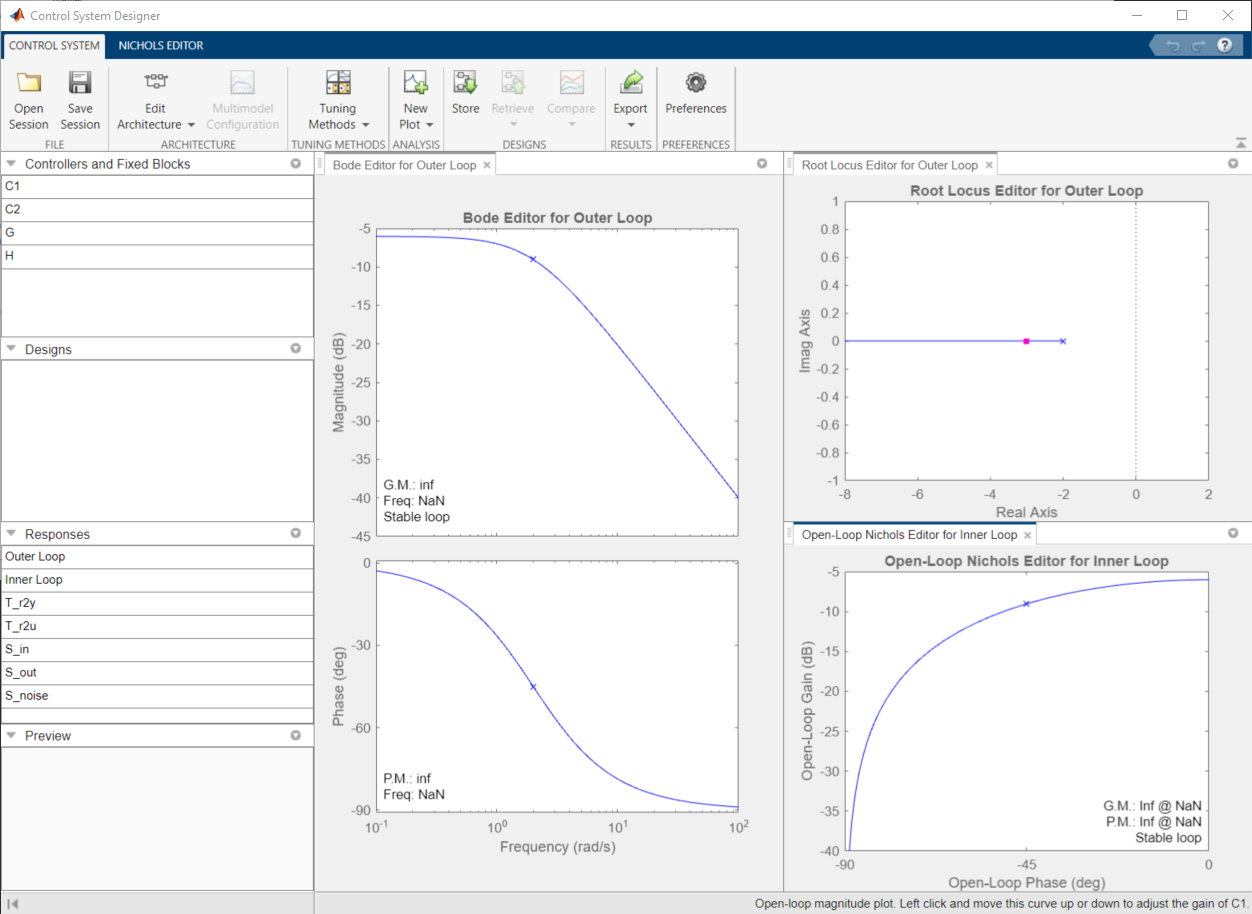
\includegraphics[width=0.65\textwidth]{controlsystem.png}
        %\caption{controlsystem.}
    \end{figure}
         
\end{frame}


\begin{frame}{Resposta ao degrau}

- Foi verificado a resposta ao degrau do sistema em malha aberta.

\begin{figure}
        \centering
        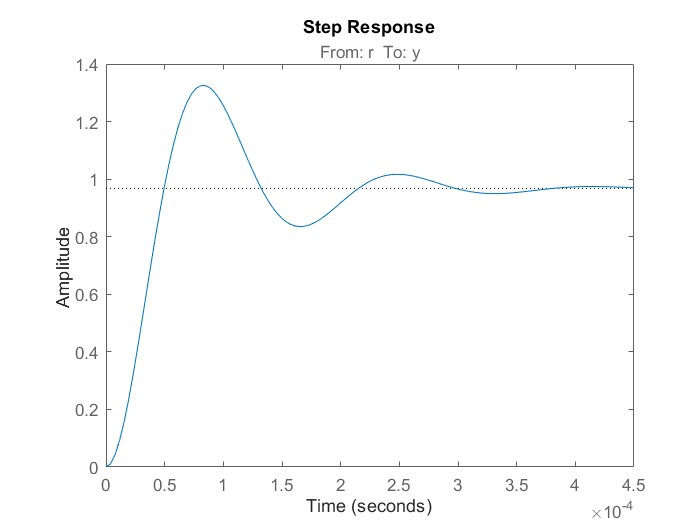
\includegraphics[width=0.65\textwidth]{respostasistemanormal.jpg}
        %\caption{Resposta ao degrau}
    \end{figure}

 
 \end{frame}

\begin{frame}{Escolha do Controlador}

\textbf{características do sistema}\\
- Sobressinal Elevado \\
 - Erro em Regime Permanente
 
    \begin{itemize}
       
        \item Foi verificado que o controlador PI é o ideal para a planta:
            \begin{itemize}
                \item A ação Integral ($K_i$) elimina o erro em regime permanente.
                \item A ação Proporcional ($K_p$) garante o tempo de resposta e o amortecimento desejados.
            \end{itemize}
        \item Os ganhos $K_p$ e $K_i$ foram ajustados diretamente pela alocação dos pólos dominantes na ferramenta gráfica.
    \end{itemize}
\end{frame}

 \begin{frame}{LGR}
 
\item O método do Lugar Geométrico das Raízes (LGR) permitiu avaliar visualmente a trajetória dos pólos e a estabilidade da malha fechada. \\

utilizando o controlSystemDesigner

 \begin{figure}

\centering
        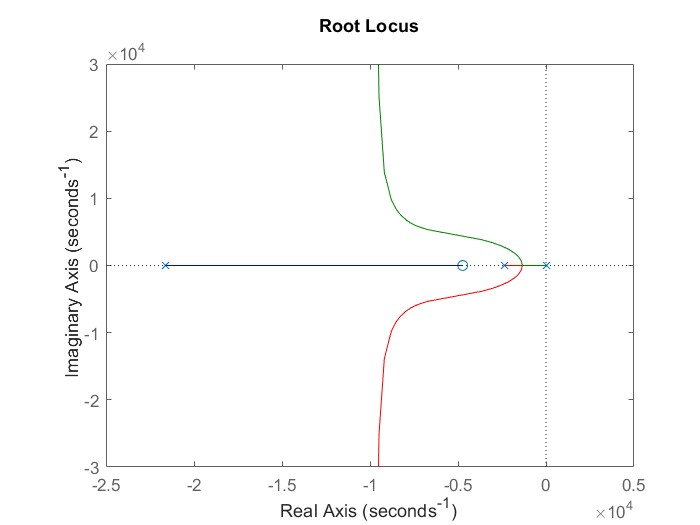
\includegraphics[width=0.5\textwidth]{rlocus.jpg}
        %\caption{LGR}
    \end{figure}
 \end{frame}


    \begin{frame}{Sintonia do Controlador PI}
\setbeamercolor{block title}{bg=black, fg=white}
  \setbeamercolor{block body}{bg=gray!10, fg=black}
  
\begin{block}{Ganhos Obtidos no MATLAB - controlSystemDesigner}
    $$C(s) = \frac{K_p\cdot s + {K_i}}{s}$$
    
    \begin{itemize}
        \item \textbf{Ganho Proporcional ($K_p$):} $0{,}0455$
        \item \textbf{Ganho Integral ($K_i$):} $215{,}0596$
    \end{itemize}
\end{block}

\end{frame}

\begin{frame}{Discretização do Controlador}
\setbeamercolor{block title}{bg=black, fg=white}
  \setbeamercolor{block body}{bg=gray!10, fg=black}
\begin{block}{Função de Transferência Discreta $G_{dc}(z)$ — Método de Tustin}
    $$G_{dc}(z) = \frac{0{,}0476 \, z - 0{,}0433}{z - 1}$$
\end{block}


\end{frame}

\begin{frame}{Resposta ao degrau}

- Resposta em malha fechada\\

 \begin{figure}

\centering
        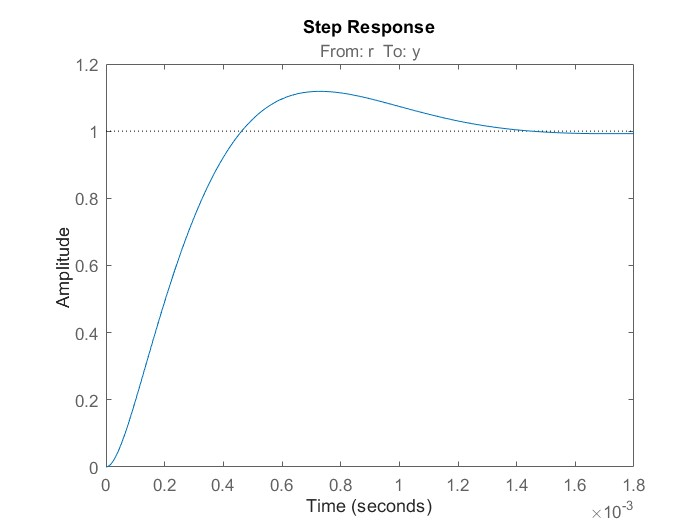
\includegraphics[width=0.65\textwidth]{respostacontrol.jpg}
        %\caption{resposta}
    \end{figure}
    
\end{frame}

\section{Conclusão e Trabalhos Futuros}
\begin{frame}{Conclusão e Trabalhos Futuros}

\setbeamercolor{block title}{bg=black, fg=white}
  \setbeamercolor{block body}{bg=gray!10, fg=black}

\begin{block}{Conclusões}
    \begin{itemize}
        \item \textbf{Modelagem e Identificação:} O modelo analítico em espaço de estados e a modelagem empírica via ARX representaram com precisão a dinâmica do conversor Buck.
        \item \textbf{Projeto do Controlador:} A sintonia do PI via LGR ($K_p = 0{,}0455$, $K_i = 215{,}0596$) garantiu estabilidade e eliminou o erro em regime permanente.
        \item \textbf{Discretização:} A conversão por Tustin permitiu obter a equação em diferenças $G_{dc}(z)$ pronta para embarcação digital.
    \end{itemize}
\end{block}
\end{frame}

\begin{frame}{Conclusão e Trabalhos Futuros}

    \setbeamercolor{block title}{bg=black, fg=white}
  \setbeamercolor{block body}{bg=gray!10, fg=black}
  
\begin{block}{Trabalhos Futuros}
    \begin{itemize}
        \item Implementação e validação de estratégias de Controle Preditivo Baseado em Modelo (MPC).
        \item Testes experimentais na bancada física do conversor Buck.
    \end{itemize}
\end{block}

\end{frame}
 
  \begin{frame}
      \titlepage
  \end{frame}

    

\end{document}